\documentclass[12pt,a4paper]{report}
\usepackage[brazil]{babel}

\usepackage[style=numeric,backend=biber]{biblatex}
\usepackage[utf8]{inputenc}
\usepackage{kpfonts}
\usepackage[T1]{fontenc}
\usepackage{wrapfig}
\usepackage{graphicx}
\usepackage{enumerate}
\usepackage{subcaption}
\usepackage{float}
\usepackage{caption}
\usepackage{listings}
\usepackage{lipsum}
\usepackage{amsthm}
\usepackage{amssymb}
\usepackage{bm}
\usepackage{color}
\usepackage{afterpage}
\usepackage[inline]{enumitem}
\usepackage{pdflscape}
\usepackage{listingsutf8}
\usepackage{siunitx}
\usepackage{bashful}

\lstset{frame=tb,
  aboveskip=2mm,
  belowskip=2mm,
  showstringspaces=false,
  columns=flexible,
  basicstyle=\footnotesize,,
  numbers=left,
  numbersep=5pt,
  stepnumber=1,
  breaklines=true,
  keepspaces=true,
  breakatwhitespace=true,
  showtabs=false,  
  tabsize=2
}


% Definindo estilo para os códigos
\definecolor{mGreen}{rgb}{0,0.6,0}
\definecolor{mGray}{rgb}{0.5,0.5,0.5}
\definecolor{mPurple}{rgb}{0.58,0,0.82}
\definecolor{dkgreen}{rgb}{0,0.6,0}
\definecolor{backgroundColour}{rgb}{0.97,0.97,0.97}

\lstdefinestyle{CStyle}{
    backgroundcolor=\color{backgroundColour},   
    commentstyle=\color{mGreen},
    keywordstyle=\color{magenta},
    numberstyle=\tiny\color{mGray},
    commentstyle=\color{dkgreen},
    stringstyle=\color{mPurple},
    basicstyle=\footnotesize,
    breakatwhitespace=false\textbf{,}         
    breaklines=true,                 
    captionpos=b,                    
    keepspaces=true,                 
    numbers=left,                    
    numbersep=5pt,                  
    showspaces=false,                
    showstringspaces=false,
    showtabs=false,                  
    tabsize=2,
    language=C
}

\lstdefinestyle{BStyle}{
    backgroundcolor=\color{backgroundColour},  
    showstringspaces=false,
    numbers=none,
    language=bash
}

\pagenumbering{arabic}
\renewcommand{\thesection}{\arabic{section}}

\bibliography{ref}
\renewcommand{\contentsname}{Sumário}{\thispagestyle{empty}}
\renewcommand{\baselinestretch}{1.5} 

\begin{document}

\begin{titlepage}
    \begin{center}
        \vspace*{1cm}
        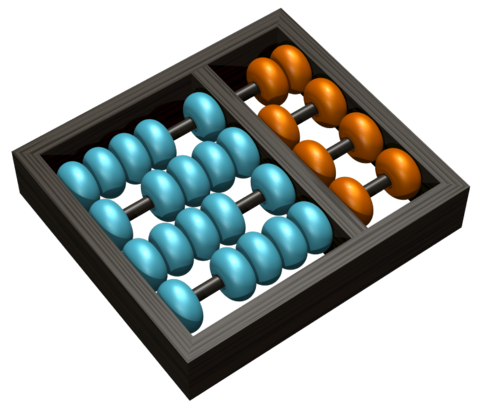
\includegraphics[width=0.25\textwidth]{Logo}\\
        \vspace{1.5cm}
        \Huge
    	\textbf{Título do Meu Relatório}\\
        \vspace{1.5cm}
        \Large
        \textbf{Alunos}: João Santos e Maria da Silva\\
        \textbf{RA}: 999991 e 999992\\
        \vspace{1.2cm}
    	\Large 
    	Instituto de Computação\\
    	Universidade Estadual de Campinas\\
    	\vspace{1.5cm}
        Campinas, 15 de Agosto de 2017.
    \end{center}
\end{titlepage}
\tableofcontents
\clearpage

\newcommand{\shellcmd}[1]{\texttt{\footnotesize\# #1}}%estilizando citação de comandos do shell

\section{Hello World!}

\subsubsection{Meu Hello World!}
Mensagem de hello world [exemplo.c:4].

\begin{lstlisting}[style=CStyle]%incluindo código no arquivo

#include <stdio.h>

#include <stdlib.h>

int main() {
    printf("Hello World!");//imprime
    return 0;
}
\end{lstlisting}

\section{Hello World Number Two!}

\subsubsection{Meu Hello World!}
Mensagem de hello world [exemplo.c:4].
\lstinputlisting[language=C, style=CStyle]{main.c}


\section{Saída do Terminal Usando NETSTAT}

Utilizando o comando \shellcmd{netstat -ut} obteve-se a seguinte saída:

\begin{lstlisting}[style=BStyle]
# netstat -ut
Active Internet connections (w/o servers)
Proto Recv-Q Send-Q Local Address           Foreign Address         State      
tcp        0      0 orion:40474             cb-in-f188.1e100.n:5228 ESTABLISHED
tcp        1      0 orion:49124             cerejeira.unicamp.:http CLOSE_WAIT 
tcp        0      0 orion:49696             104.20.110.39:https     ESTABLISHED
tcp        0      0 orion:44318             104.19.194.102:https    ESTABLISHED
tcp        1      0 orion:49134             cerejeira.unicamp.:http CLOSE_WAIT 
tcp        0      0 orion:59136             23.99.92.253:https      ESTABLISHED
tcp        0      0 orion:43240             172.217.29.110:https    ESTABLISHED
tcp        1      0 orion:49120             cerejeira.unicamp.:http CLOSE_WAIT 
tcp        1      0 orion:49118             cerejeira.unicamp.:http CLOSE_WAIT 
tcp        1      0 orion:49850             45.55.41.223:http       CLOSE_WAIT 
tcp        0      0 orion:48268             a1.ue.vip.bf1.yah:https ESTABLISHED
tcp   390280      0 orion:49122             cerejeira.unicamp.:http ESTABLISHED
tcp        1      0 orion:49132             cerejeira.unicamp.:http CLOSE_WAIT 
udp        0      0 orion:55918             172.217.29.110:https    ESTABLISHED
udp        0      0 orion:56147             172.217.29.106:https    ESTABLISHED
udp        0      0 orion:49038             172.217.29.131:https    ESTABLISHED
udp        0      0 orion:49805             rio01s16-in-f99.1:https ESTABLISHED
udp        0      0 orion:42003             172.217.29.110:https    ESTABLISHED
udp        0      0 orion:52637             172.217.29.138:https    ESTABLISHED
\end{lstlisting}

% \printbibliography%caso tiver referências, usar arquivo .bib para por as referências, descomente quando precisar :)

\section{Saída do Terminal Usando ARP}

Utilizando o comando \shellcmd{arp} obteve-se a seguinte saída:

\begin{lstlisting}[style=BStyle]
# arp
arp
Address                  HWtype  HWaddress           Flags Mask            Iface
192.168.0.3                      (incomplete)                              enp2s0
192.168.0.112                    (incomplete)                              enp2s0
gateway                  ether   8c:04:ff:21:a9:92   C                     enp2s0
192.168.0.115                    (incomplete)                              enp2s0
192.168.0.19                     (incomplete)                              enp2s0
192.168.0.132                    (incomplete)                              enp2s0
192.168.0.12             ether   30:f9:ed:c7:ea:12   C                     enp2s0
192.168.0.15             ether   ec:08:6b:96:17:70   C                     enp2s0
192.168.0.8                      (incomplete)                              enp2s0
192.168.0.101                    (incomplete)                              enp2s0
192.168.0.11             ether   c4:3a:be:cf:cf:bc   C                     enp2s0
192.168.0.10             ether   08:3e:8e:d1:39:a7   C                     enp2s0
192.168.0.103                    (incomplete)                              enp2s0
192.168.0.4                      (incomplete)                              enp2s0
192.168.0.1                      (incomplete)                              enp2s0

\end{lstlisting}

\end{document}